% $Header: /cvsroot/latex-beamer/latex-beamer/solutions/conference-talks/conference-ornate-20min.en.tex,v 1.6 2004/10/07 20:53:08 tantau Exp $

\documentclass[11pt,table]{beamer}
\usepackage{xcolor}
% This file is a solution template for:

% - Talk at a conference/colloquium.
% - Talk length is about 20min.
% - Style is ornate.

% Copyright 2004 by Till Tantau <tantau@users.sourceforge.net>.
%
% In principle, this file can be redistributed and/or modified under
% the terms of the GNU Public License, version 2.
%
% However, this file is supposed to be a template to be modified
% for your own needs. For this reason, if you use this file as a
% template and not specifically distribute it as part of a another
% package/program, I grant the extra permission to freely copy and
% modify this file as you see fit and even to delete this copyright
% notice. 
\usepackage{color}

%\usepackage{wasysym}
%\usepackage{movie15} 
\newcommand{\red}[1]{\textcolor{red}{#1}}
\newcommand{\green}[1]{\textcolor{green}{#1}}
\usepackage{tikz}
\usetikzlibrary{bayesnet}

\definecolor{curie}{rgb}{1,0.4,0}

% pastel colors (latent nodes)
\definecolor{lavender}{rgb}{0.67,0.5,1.0}
\definecolor{cream}{rgb}{0.96,0.8,0.69}
\definecolor{tomato}{rgb}{1.0,0.41,0.41}
\definecolor{lightpink}{rgb}{1.0,0.75,0.796}
\definecolor{SpringGreen}{rgb}{0.5,1.0,0}
\definecolor{anis}{rgb}{0.858,0.858,0.44}
\definecolor{lightBlue}{rgb}{0.59,1.0,1.0}
\definecolor{blue}{rgb}{0.36,0.67,0.93}


% dark colors (observed nodes)
\definecolor{DarkViolet}{rgb}{0.28,0.24,0.545}
\definecolor{DarkBlue}{rgb}{0.06,0.3,0.545}
\definecolor{DarkRed}{rgb}{0.545,0.137,0.137}
\definecolor{DarkBrown}{rgb}{0.36,0.2,0.09}
\definecolor{DarkGreen}{rgb}{0,0.39,0}
\definecolor{DarkPink}{rgb}{0.545,0.04,0.31}


\tikzset{
  treenode/.style = {align=center, inner sep=0pt, text centered,
    font=\sffamily},
  grey_node/.style = {treenode, circle, white, font=\sffamily\bfseries, draw=black,
    fill=grey, text width=1.5em},% noeud gris (observation)
  red_node/.style = {treenode, circle, red, draw=red, 
    text width=1.5em, very thick},% noeud rouge (paramètre)
 white_node/.style = {treenode, circle, black, draw=black, 
    text width=1.5em, very thick},% noeud rouge (paramètre)
  arn_x/.style = {treenode, rectangle, draw=black,
    minimum width=0.5em, minimum height=0.5em}% arbre rouge noir, nil
}

\usetikzlibrary{positioning,shapes,shadows,arrows}

% couleur curie

  \usetheme{Boadilla}
  % or ...

  \setbeamercovered{transparent}
  % or whatever (possibly just delete it)

\setbeamertemplate{navigation symbols}{}

\usepackage[utf8]{inputenc} 	% L'encodage. Ca peut être à remplacer par \usepackage[utf8]{inputenc}
\usepackage[T1]{fontenc}
\def\ques{\noindent{\bf Question : }}
\usepackage[english]{babel}

\usepackage[utf8]{inputenc}
% or whatever

\usepackage{times}
\usepackage[T1]{fontenc}
% Or whatever. Note that the encoding and the font should match. If T1
% does not look nice, try deleting the line with the fontenc.
\usepackage{graphics}

\title % (optional, use only with long paper titles)
{Estimation par maximum de vraisemblance composite des paramètres du modèle Poisson log-normal}

\subtitle{Mémoire de M2 réalisé sous la supervision de Stéphane Robin}

\author[Elsa TEULIERE] % (optional, use only with lots of authors)
{Elsa TEULIERE}
% - Give the names in the same order as the appear in the paper.
% - Use the \inst{?} command only if the authors have different
%   affiliation.

\institute[UPMC] % (optional, but mostly needed)
{
%   \inst{1}%
%    UMR144 Institut Curie, CNRS
%   \and
  Master 2 Probabilités et modèles aléatoires}
% - Use the \inst command only if there are several affiliations.
% - Keep it simple, no one is interested in your street address.

\date[\today] % (optional, should be abbreviation of conference name)
{\today}
% - Either use conference name or its abbreviation.
% - Not really informative to the audience, more for people (including
%   yourself) who are reading the slides online

% This is only inserted into the PDF information catalog. Can be left
% out. 


% If you have a file called "university-logo-filename.xxx", where xxx
% is a graphic format that can be processed by latex or pdflatex,
% resp., then you can add a logo as follows:

% \logo{\pgfuseimage{curie-logo}}



% Delete this, if you do not want the table of contents to pop up at
% the beginning of each subsection:


%\AtBeginSubsection[]
%{
%  \begin{frame}<beamer>
%    \frametitle{Outline}
%    \tableofcontents[currentsection,currentsubsection]
%  \end{frame}
%}


% If you wish to uncover everything in a step-wise fashion, uncomment
% the following command: 

%\beamerdefaultoverlayspecification{<+->}
\graphicspath{ {./figures/} }


\begin{document}

\begin{frame}
  \titlepage

\end{frame}
\section*{Introduction}

\begin{frame}
\frametitle{Etude d'un réseau d'interaction}
%\vspace{1cm}
\begin{figure}
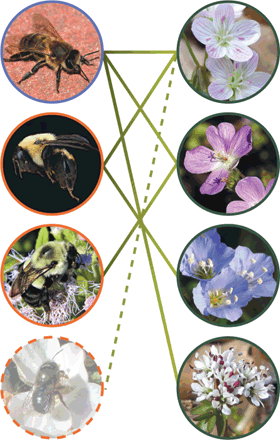
\includegraphics[scale=0.3]{Plant_polinisator.png}
\caption{Exemple d'un réseau plantes-pollinisateurs} 
\end{figure}
\end{frame}

\section{Le modèle Poisson log-normal}
\begin{frame}
\frametitle{Le modèle Poisson log-normal}
$(\mu, \Sigma) \in \mathbb{R}^n \times \mathcal{M}_n(\mathbb{R})$\\
\vspace{0.5cm}

$(Y_1,...,Y_n) \sim \mathcal{PLN} (\mu,\Sigma)$  \\

\begin{itemize}
\item  $Z \sim \mathcal{N}_n(0,\Sigma)$ une variable gaussienne  latente

\item$\forall i \in \{1,...,n\}, Y_i\mid Z_i \sim \mathcal{P}(\mathrm{exp}(\mu_i+Z_i))$

\item $(Y_i\mid Z )_{i \in \{1,...,n\}}$ sont indépendantes.
\end{itemize}
\end{frame}
\subsection{Avec les covariables et le offset}

\begin{frame}
\frametitle{Le modèle Poisson log-normal avec les covariables}
$X \in \mathbb{R}^d$ le vecteur de covariables.\\
$O \in \mathbb{R}^n$ le vecteur d'offset.\\
\vspace{0.5cm}
$(M, \Sigma) \in \mathcal{M}_{d \times n}(\mathbb{R}) \times \mathcal{M}_n(\mathbb{R})$\\
\vspace{0.5cm}
$(Y_1,...,Y_n) \sim \mathcal{PLN}_X (M,\Sigma)$  \\

\begin{itemize}
\item  $Z \sim \mathcal{N}_n(0,\Sigma)$ une variable gaussienne  latente

\item$\forall i \in \{1,...,n\}, Y_i\mid Z_i \sim \mathcal{P}(\mathrm{exp}(O_i+X^T M^{(i)}+Z_i))$

\item $(Y_i\mid Z )_{i \in \{1,...,n\}}$ sont indépendantes.
\end{itemize}
\end{frame}

\subsection{Estimation des paramètres de la loi Poisson log-normale}
\begin{frame}
\frametitle{Estimation des paramètres de la loi Poisson log-normale :}
\begin{itemize}
\item \textbf{Maximum de vraisemblance :} densité de $\mathcal{PLN}(M,\Sigma)$ : $h_{(M,\Sigma)}(Y_1,...,Y_n) = \int_{\mathbb{R}^n} \prod_{i=1}^n f_{(e^{O_i+X^T M^{(i)} + z_i})}(Y_i) g_{(0,\Sigma)}(z_1...z_n) \mathrm{d}z_1...\mathrm{d}z_n$.
\item \textbf{EM :} Pas de forme explicite de $p_{(\widehat{M},\widehat{\Sigma})}(Z_i \mid Y_i)$ (\cite{Karlis2005})
\item \textbf{VEM :} Algorithme efficace mais pas de garantie assymptotique (\cite{Chiquet2017variational})
\end{itemize}
\end{frame}

\section{Composite likelihood}

\begin{frame}
\frametitle{Vraisemblance composite \cite{varin2008composite}}
\begin{center}
$\mathcal{CL}(Y)= \sum_{1\leq i <k \leq n} \mathrm{log} (h_{(M,\Sigma)}(Y_i,Y_k))$
\end{center}
 Fonction de densité en dimension 2 $ \longrightarrow $ intégrale sur $\mathbb{R}^2$.\\
\vspace{0.5cm}
Si on considère $N$ observations indépendantes et identiquement distribuées, on a :
\begin{center}
$\mathcal{CL}(Y)= \frac{1}{N}\sum_{j=1}^N \sum_{1\leq i <k \leq n} \mathrm{log} (h_{(M,\Sigma)}(Y^j_i,Y^j_k))$
\end{center}

$\rightarrow$ Estimateur par maximum de la vraisemblance composite. Consistance ? Normalité assymptotique ?
\end{frame}
\subsection{M-estimator}
\begin{frame}
\frametitle{Rappel sur les M-estimateurs : }
Un M-estimateur maximise une fonction de la forme 
\begin{center}
$\mathcal{M}_N : \theta \mapsto \frac{1}{N} \sum_{j=1}^N m_\theta(Y^j)$
\end{center}
Ici :  $m_\theta(Y^j) = \sum_{0 \leq i < k \leq n} \mathrm{log} ( h_{(M,\Sigma)}(Y_i^j,Y_k^j) )$
\end{frame}

\begin{frame}
\frametitle{Rappel sur les M-estimateurs : }
Un M-estimateur maximise une fonction de la forme 
\begin{center}
$\mathcal{M}_N : \theta \mapsto \frac{1}{N} \sum_{j=1}^N \sum_{0 \leq i < k \leq n} \mathrm{log} ( h_{(M,\Sigma)}(Y_i^j,Y_k^j) )$
\end{center}
\begin{theorem} \label{ThMest} \cite{vaart_1998}
Let $(\mathrm{M}_N)$ be a random sequence of functions in the variable $\theta$ and $M$ a determinist function in the variable $\theta$. If :
\begin{enumerate}
\item $\underset{\theta \in \Theta}{\mathrm{sup}} \mid \mathrm{M}_N(\theta)-\mathrm{M}(\theta) \mid \overset{\mathbb{P}}{\longrightarrow} 0$
\item the maximum $\theta^\ast$ of M is unique.
\end{enumerate}
Then any sequence of estimators $\widehat{\theta}_N$ with $\mathrm{M}_N(\widehat{\theta}_N) \geq \mathrm{M}_N(\theta^\ast)-\circ_p(1)$ converges in probability to $\theta^\ast$.
\end{theorem}

\end{frame}

\begin{frame}
\frametitle{Consistance du maximum de la vraisemblance composite pour le modèle poisson log normal}
\begin{theorem}
The estimator $(\widehat{M}_N,\widehat{\Sigma}_N)$ constructed by maximizing the composite pairwise likelihood for $(Y^j_1,...Y^j_n)_{j \in \{1...N\}}$ is a consistent estimator of the correlation coefficients $M^\ast$ and of the matrix of variance-covariance $\Sigma^\ast$.
\end{theorem}
\end{frame}
\begin{frame}
\begin{proof}
\begin{enumerate}
\item Par la LFGN :
\begin{align*}
\underset{(M,\Sigma)}{\mathrm{sup}} \mid \mathcal{M}_N(M, \Sigma)- \mathbb{E}_X [\sum_{1 \leq i <k \leq n} \mathbb{E}_{Y_i,Y_k \mid X} [ \mathrm{log}(h_{(M,\Sigma \mid X)} (Y_i,Y_k))]] \mid\overset{\mathbb{P}}{\longrightarrow}  0
\end{align*} 
\item Existence et unicité du maximum de $\mathcal{M}(M,\Sigma) = \mathbb{E}_X [\sum_{1 \leq i < k \leq n} \mathbb{E}_{Y_i,Y_k \mid X} [ \mathrm{log}(h_{(M,\Sigma \mid X)} (Y_i,Y_k))]]$.
\begin{itemize}
\item Identifiabilité du modèle (par les moments)
\item Existence d'un maximum (divergence de Kullback)
\end{itemize}
\item Par construction des estimateurs : 
\begin{align*}
\forall N \in \mathbb{N},  \mathcal{M}_N(\widehat{M}_N, \widehat{\Sigma}_N) \geq \mathcal{M}_N(M^\ast, \Sigma^\ast) 
\end{align*}
\end{enumerate}
\end{proof}
\end{frame}
\begin{frame}
\begin{proof}
\begin{itemize}
\item Identifiabilité du modèle \\
On rappelle les moments de la loi Poisson log-normale :
\begin{align*}
\mathbb{E}_{(M,\Sigma \mid X)} [Y_i] &= \mathrm{exp}(O_i + X^T M^{(i)} + \frac{1}{2} \sigma_{ii} )\\
\mathbb{V}_{(M,\Sigma \mid X)} [Y_i]& =\mathbb{E}_{(M,\Sigma \mid X)} [Y_i]+\mathbb{E}_{(M,\Sigma \mid X)} [Y_i]^2(\mathrm{exp}(\sigma_{ii})-1)\\
\mathrm{Cov}(Y_i,Y_k)& =\mathbb{E}_{(M,\Sigma \mid X)} [Y_i]\mathbb{E}_{(M,\Sigma \mid X)} [Y_k](\mathrm{exp}(\sigma_{ik}) - 1)
\end{align*}
Soit $(M,\Sigma)$ et $(M', \Sigma')$ tels que pour tout $X \in \mathcal{X}$,$\mathcal{PLN}_X(M,\Sigma)\sim \mathcal{PLN}_X(M',\Sigma')$. Par égalité des moments on a :
\begin{itemize}
\item $ \forall i \in \{1...n\}$, $\sigma_{ii} = \sigma'_{ii}$.
\item $\forall (i,k) \in \{1..n\}^2$, $\sigma_{ik} = \sigma'_{ik}$
\item  $ \forall i \in \{1...n\}$, $ \forall X \in \mathcal{X}$, $X^T (M^{(i)}-M'^{(i)})=0$\\
\textit{ie} si $\mathcal{X}= \mathbb{R}^d$, $M^{(i)} = M'^{(i)}$.
\end{itemize}
\end{itemize}
\end{proof}
\end{frame}
\begin{frame}
\begin{proof}
\begin{itemize}
\item Existence d'un maximum \\
On rappelle la définition de la divergence de Kullback :
\begin{align*}
\mathrm{D_{KL}}(p_{\theta^\ast} \parallel p_{\theta})= \int p_{\theta^\ast}(x) \mathrm{log}(\frac{p_{\theta^\ast}(x)}{p_{\theta}(x)}) \mathrm{d}x
\end{align*}
On a 
\begin{align*}
\mathbb{E}_X[\mathbb{E}_{(M^{\ast},\Sigma^{\ast} \mid X)}&[\mathrm{log}(h_{(M^{\ast},\Sigma^{\ast} \mid X)}(Y_i,Y_k)) - \mathrm{log}(h_{(M,\Sigma\mid X)}(Y_j,Y_k))]] \\
& = \mathbb{E}_X[\mathrm{D_{KL}}(h_{(M^\ast,\Sigma^\ast \mid X)}\parallel h_{(M,\Sigma \mid X)})]\\
& = \mathbb{E}_X[\mathbb{E}_{(M^{\ast},\Sigma^{\ast} \mid X)}[\mathrm{log}(h_{(M^{\ast},\Sigma^{\ast} \mid X)}(Y_i,Y_k))]] - \mathrm{M}(M,\Sigma)
\end{align*}
Maximiser la vraisemblance composite revient à minimiser la divergence de Kullback. \
$\mathrm{D_{KL}} \geq 0$, 
\begin{align*}
\mathrm{D_{KL}}(h_{(M^\ast,\Sigma^\ast \mid X)}\parallel h_{(M,\Sigma \mid X)}) = 0 
\Leftrightarrow
(M,\Sigma) = (M^\ast, \Sigma^\ast)
\end{align*}

\end{itemize}
\end{proof}
\end{frame}
\begin{frame}
\frametitle{Normalité assymptotique}
 $(\widehat{M}_N,\widehat\Sigma_N)$ est une suite d'estimateurs consistant du maximum $(\widehat{M}^\ast,\widehat{\Sigma}^\ast)$ de la fonction $\mathcal{M}(M,\Sigma) = \mathbb{E}_X [\mathbb{E}_{Y_i,Y_k \mid X} [ \mathrm{log}(h_{(M,\Sigma \mid X)} (Y_i,Y_k))]]$.\\
\vspace{0.5cm}
 
Par la théorie des M-estimateurs \cite{vaart_1998}, sous des conditions de régularités de $\mathcal{M}$ :\\
\begin{center}
$ \sqrt{n}((\widehat{M}_N,\widehat\Sigma_N) - (\widehat{M}^\ast,\widehat{\Sigma}^\ast)) \overset{\mathcal{L}}{\longrightarrow} \mathcal{N}(0, \mathbb{E}[\ddot{\mathcal{M}}(M^\ast, \Sigma^\ast)]^{-1} \mathbb{E}[ \dot{\mathcal{M}}(M^\ast,\Sigma^\ast) \dot{\mathcal{M}}(M^\ast,\Sigma^\ast)^T ]\mathbb{E}[\ddot{\mathcal{M}}(M^\ast, \Sigma^\ast)]^{-1} ) $
\end{center}
\begin{itemize}
\item Calcul du gradient et de la matrice hessienne pour estimer la variance de la normalité assymptotique.
\end{itemize}
 
\end{frame}
\begin{frame}
\frametitle{Résultats de simulation}
\begin{figure}
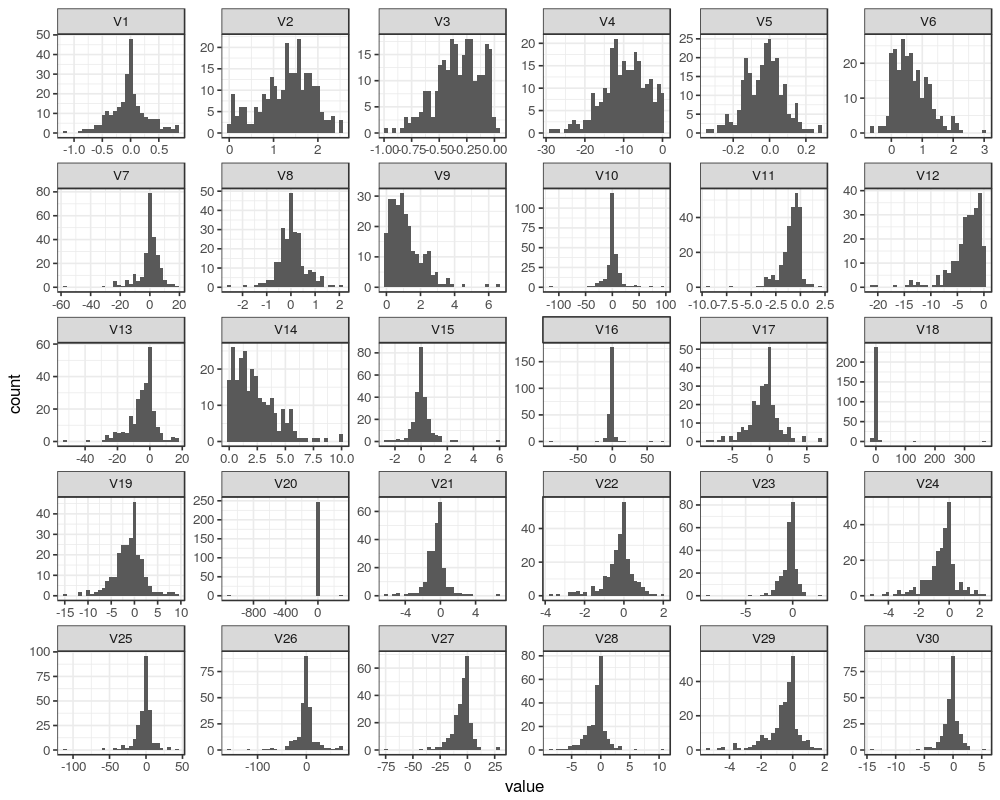
\includegraphics[scale=0.3]{graph53_st_DIRETC_L.png}
\caption{Resultats normalisés de l'estimation des paramètres d'une loi Poisson log-normale pour 5 espèces et 3 covariables sur 100 échantillonages. Simulations répétées 250 fois. }
\end{figure}
\end{frame}




\begin{frame}
\frametitle{Dépendance spatiale : Estimer $\Gamma$}
\begin{figure}
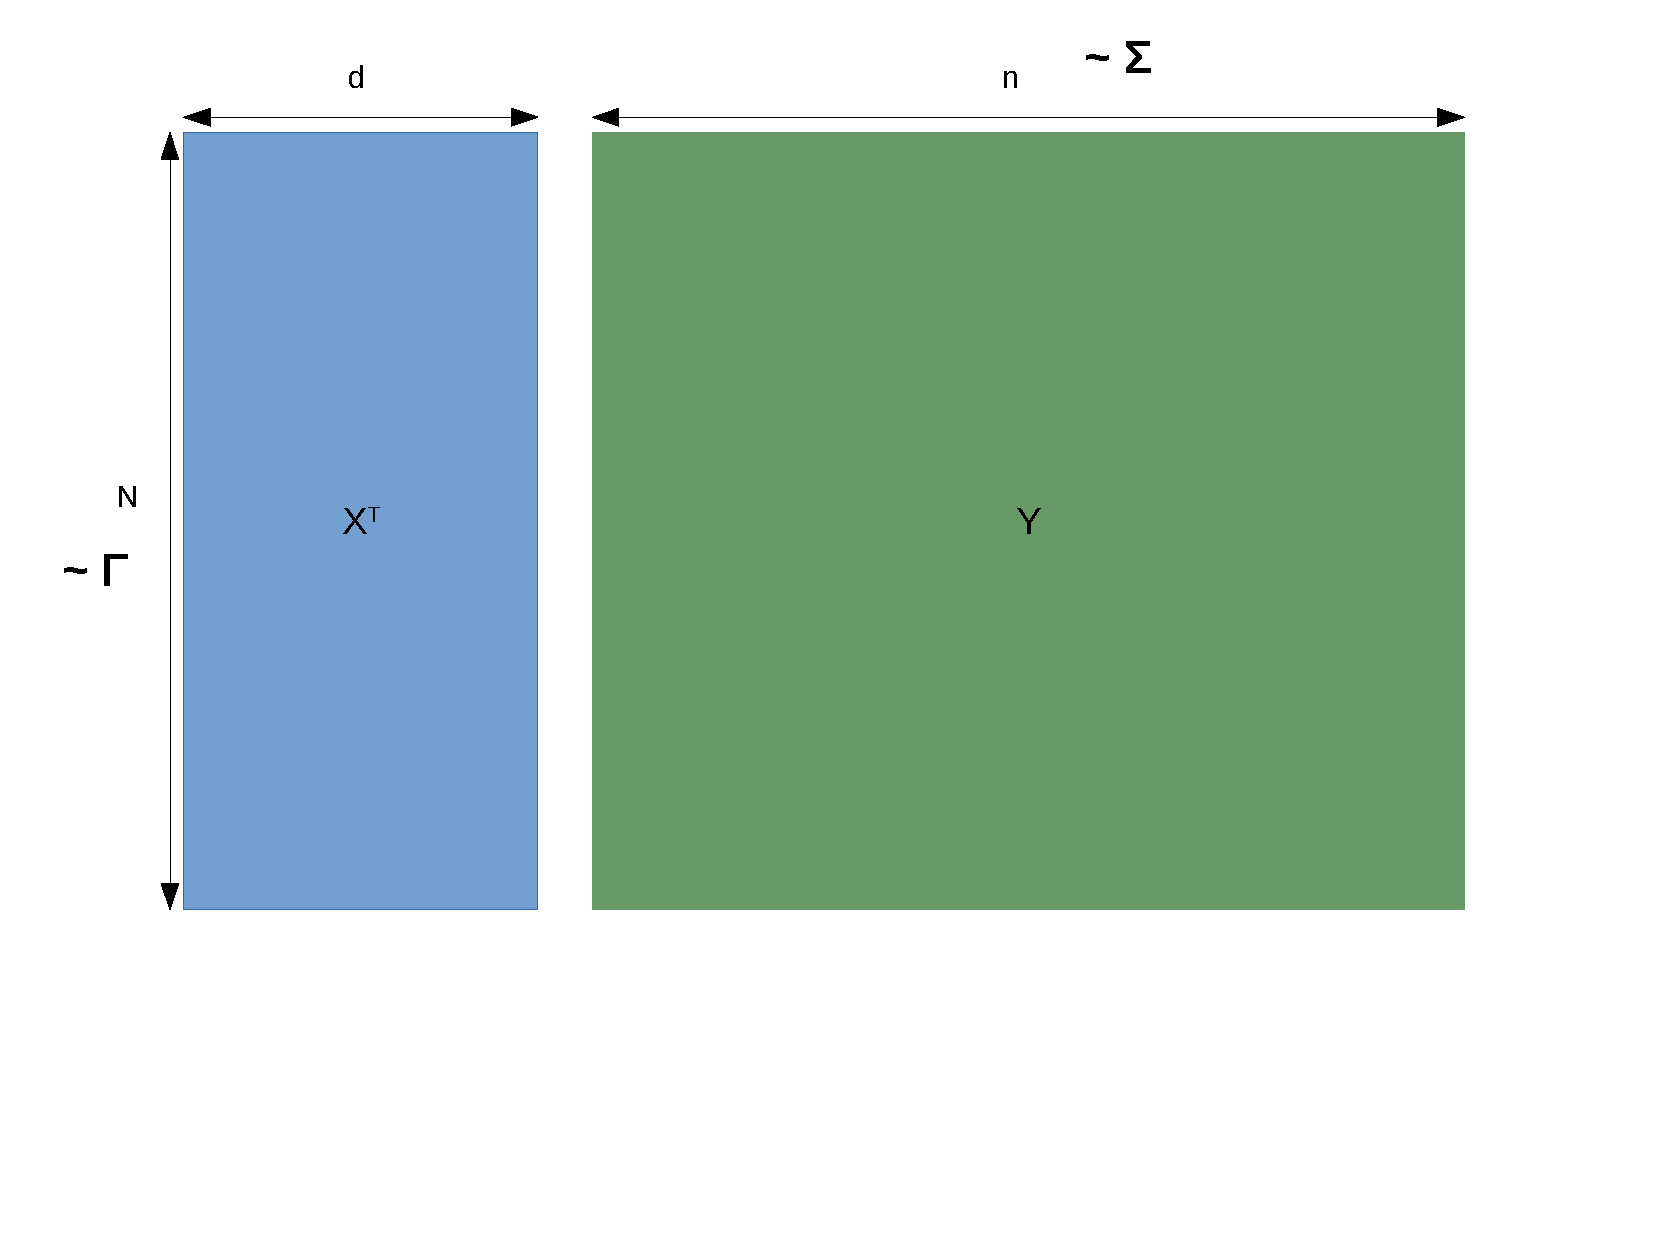
\includegraphics[scale=0.3]{Dependance_2.pdf}
\end{figure}
\end{frame}

\begin{frame}
\frametitle{Dépendance spatiale : Estimer $\Gamma$}
       \begin{tabular}{cl}  
         \begin{tabular}{c}
           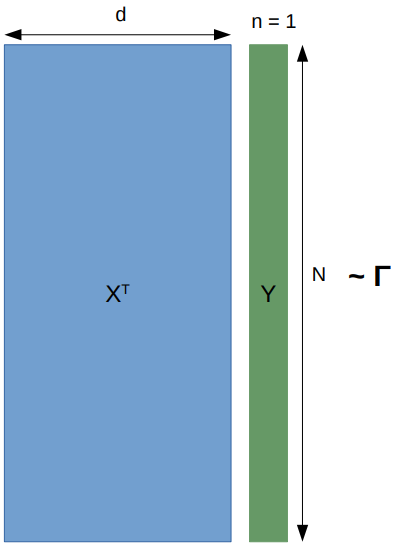
\includegraphics[scale=0.3]{Spatiales.png}
           \end{tabular}
           & \begin{tabular}{l}
             \parbox{0.5\linewidth}{%  change the parbox width as appropiate
             $ Z \sim \mathcal{N}_N(0,\Gamma)$ variable latente\\
             \vspace{1cm}
             
             $ Y^j\mid Z^j \sim \mathcal{P}(e^{O_j+\beta^T X_j + Z_j})$\\
             \vspace{1cm}
             
             $\mathcal{CL}_{(M^T, \Gamma)}(Y) = \sum_{1 \leq j < l\leq N} \mathrm{log}(h_{(M^T,\Gamma)} (Y^j,Y^l) )$
    }
         \end{tabular}  \\
\end{tabular}


\end{frame}


\begin{frame}
\frametitle{Double dépendance : Estimer $\Gamma$ et $\Sigma$}
       \begin{tabular}{cl}  
         \begin{tabular}{c}
           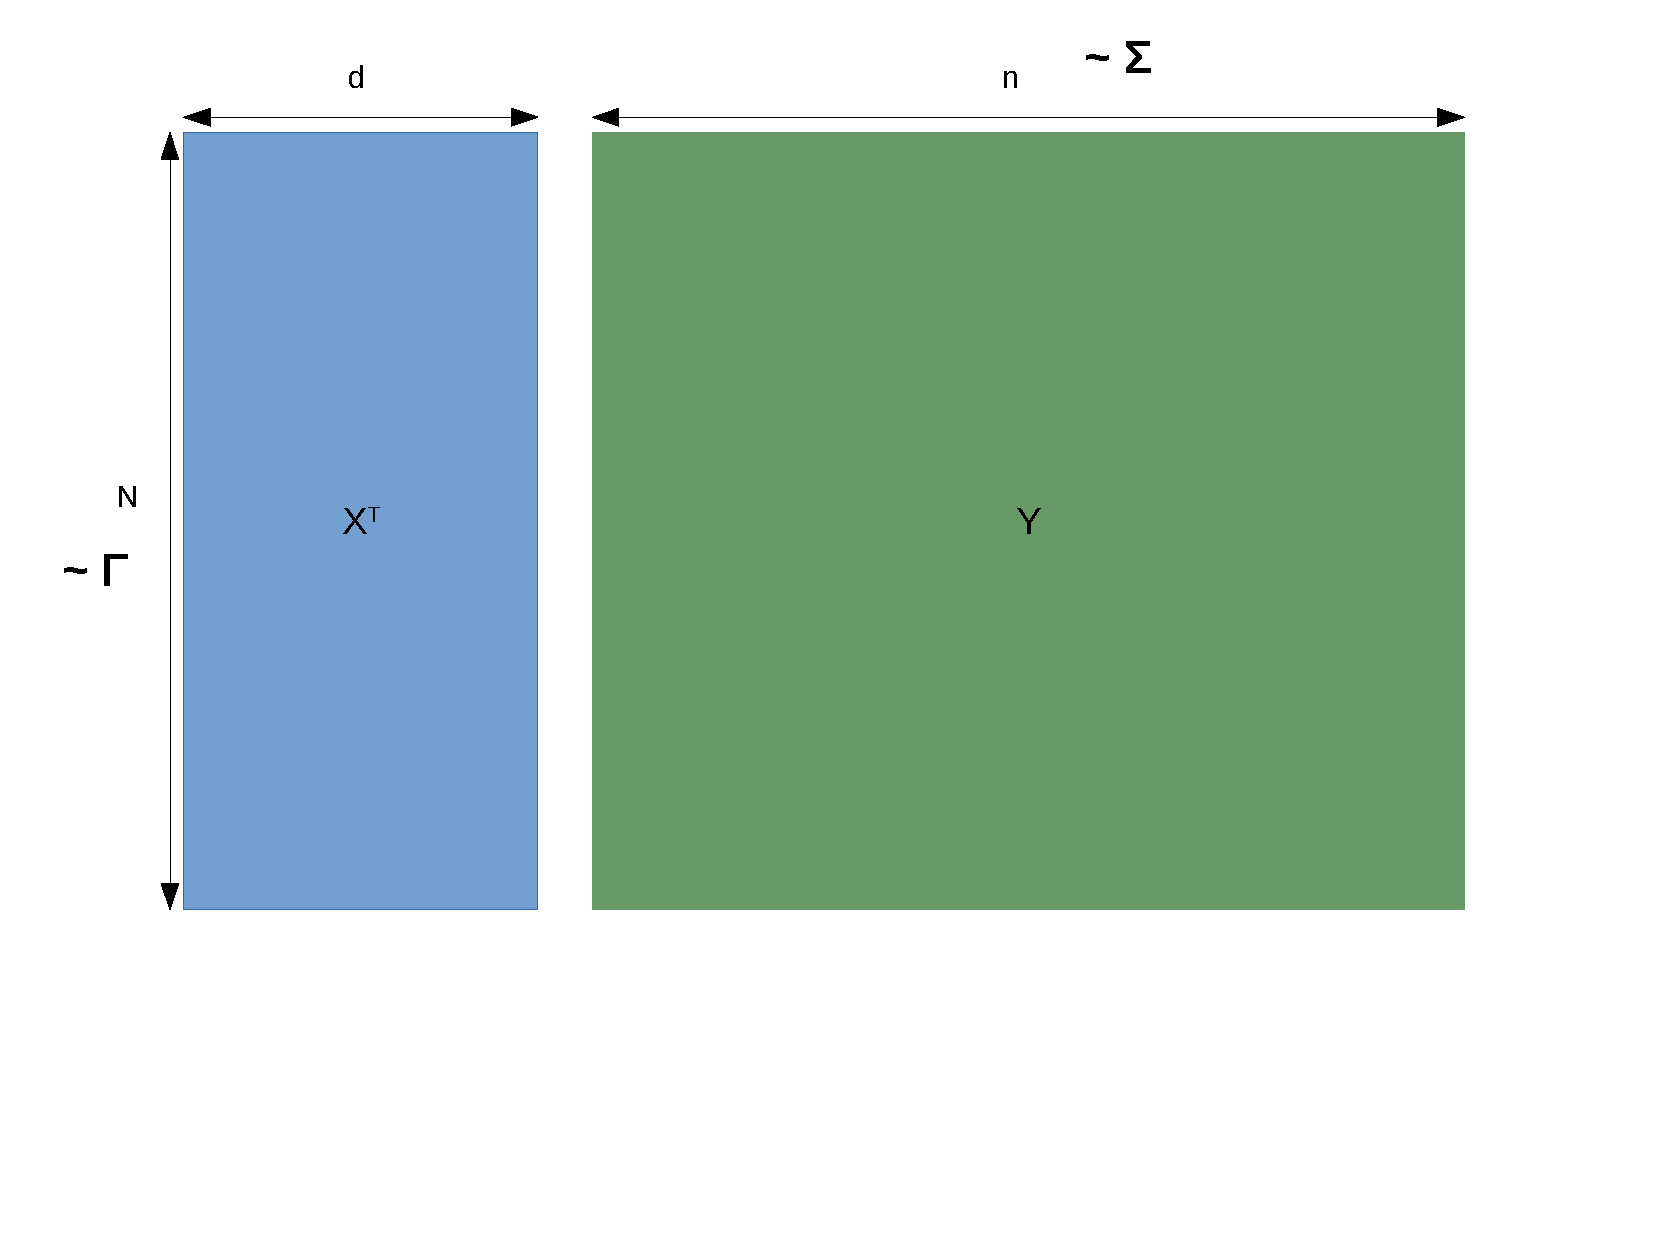
\includegraphics[scale=0.2]{Dependance_2.pdf}
           \end{tabular}
           & \begin{tabular}{l}
             \parbox{0.5\linewidth}{%  change the parbox width as appropiate
             $ \mathbb{V} (Y) = \Gamma \otimes \Sigma$ \\
             \vspace{1cm}
             
             Maximiser\\
              $\mathcal{CL}_{(M,\Sigma)} + \mathcal{CL}_{(M^T, \Gamma)}$
    }
         \end{tabular}  \\
\end{tabular}


\end{frame}




\begin{frame}

\frametitle{Conclusion}
\begin{itemize}
\item Modèle Poisson log-normal pertinent pour modéliser des données avec dépendances
\item Construction d'un estimateur en maximisant 
\begin{align*}
\mathcal{CL}(Y)= \frac{1}{N}\sum_{j=1}^N \sum_{1\leq i <k \leq n} \mathrm{log} (h_{(M,\Sigma)}(Y^j_i,Y^j_k))
\end{align*}
\item estimateur consistant et (surement) assymptotiquement normal
\item adaptation au cas de la dépendance spatiale
\end{itemize}
\end{frame}

\begin{frame}
\begin{center}
Merci pour votre attention ! 
\end{center}
\end{frame}

\begin{frame}
\frametitle{Dans le cas d'une dépendance structurée}
On suppose :
\begin{align*}
\Sigma = \sigma^2 \begin{pmatrix}
1 &  e^{-\alpha d_{1,2}} &  e^{-\alpha d_{1,2}} & \ldots &  e^{- \alpha d_{1,n}}  \\
 e^{-\alpha d_{1,2}} & 1 & \ldots & \ldots &  e^{- \alpha d_{2,n}}\\
 \vdots & & \ddots & & \vdots\\
 \vdots & & & \ddots & \vdots \\
 e^{-\alpha d_{1,n}} &  e^{-\alpha d_{2,n}} & \ldots & \ldots & 1 
\end{pmatrix}
\end{align*} 
Dans ce cas : $h_{(M,\alpha,\sigma^2)}$
\end{frame}

\begin{frame}
\frametitle{Dans le cas d'une dépendance structurée}
\begin{itemize}
\item $\mathcal{CL}^I = \sum_{(i,j) \in I} \mathrm{log}( h_{(M^{(ij)},\alpha,\sigma^2)}(Y_i,Y_j)) $
 \item Par regression linéaire on a 
\begin{align*}
\mathrm{log}(\widehat{\sigma_{ij}}) = \mathrm{log} ( \sigma^2) - \alpha d_{ij} + E_{ij}
\end{align*}

\item De plus\begin{align*}
\mathbb{V}(\widehat{\alpha}) = \rho^2 (\frac{1}{n^2} + \frac{\bar{d}^2}{\sum_{(i,j)\in \{1..n\}^2}(d_{ij} - \bar{d})^2})
\end{align*}
\item chercher un arbre couvrant maximal : algorithme de Kruskal \cite{Kruskal1956}.
\end{itemize}
\end{frame}

\bibliographystyle{plain}
\bibliography{Biblio.bib}

\end{document}